\documentclass[12pt]{article}

\usepackage{answers}
\usepackage{setspace}
\usepackage{graphicx}
\usepackage{enumitem}
\usepackage{multicol}
\usepackage{mathrsfs}
\usepackage[margin=1in]{geometry} 
\usepackage{amsmath,amsthm,amssymb}
\usepackage[ngerman]{babel}

\newcommand{\N}{\mathbb{N}}
\newcommand{\Z}{\mathbb{Z}}
\newcommand{\C}{\mathbb{C}}
\newcommand{\R}{\mathbb{R}}

\DeclareMathOperator{\sech}{sech}
\DeclareMathOperator{\csch}{csch}

\newenvironment{theorem}[2][Theorem]{\begin{trivlist}
		\item[\hskip \labelsep {\bfseries #1}\hskip \labelsep {\bfseries #2.}]}{\end{trivlist}}
\newenvironment{definition}[2][Definition]{\begin{trivlist}
		\item[\hskip \labelsep {\bfseries #1}\hskip \labelsep {\bfseries #2.}]}{\end{trivlist}}
\newenvironment{proposition}[2][Proposition]{\begin{trivlist}
		\item[\hskip \labelsep {\bfseries #1}\hskip \labelsep {\bfseries #2.}]}{\end{trivlist}}
\newenvironment{lemma}[2][Lemma]{\begin{trivlist}
		\item[\hskip \labelsep {\bfseries #1}\hskip \labelsep {\bfseries #2.}]}{\end{trivlist}}
\newenvironment{exercise}[2][Exercise]{\begin{trivlist}
		\item[\hskip \labelsep {\bfseries #1}\hskip \labelsep {\bfseries #2.}]}{\end{trivlist}}
\newenvironment{solution}[2][Solution]{\begin{trivlist}
		\item[\hskip \labelsep {\bfseries #1}]}{\end{trivlist}}
\newenvironment{problem}[2][Problem]{\begin{trivlist}
		\item[\hskip \labelsep {\bfseries #1}\hskip \labelsep {\bfseries #2.}]}{\end{trivlist}}
\newenvironment{question}[2][Question]{\begin{trivlist}
		\item[\hskip \labelsep {\bfseries #1}\hskip \labelsep {\bfseries #2.}]}{\end{trivlist}}
\newenvironment{corollary}[2][Corollary]{\begin{trivlist}
		\item[\hskip \labelsep {\bfseries #1}\hskip \labelsep {\bfseries #2.}]}{\end{trivlist}}

\begin{document}
	\title{Interaktive Computergrafik}
	\author{Michael Gabler}
	\maketitle
	\tableofcontents
	\newpage

	\section{Grundlagen}
	Computergrafik beschreibt das Erstellen von 2D-Bildern aufgrund von 3D-Daten.\\
	\textbf{Anwendungsgebiete}
	\begin{itemize}
		\item Human-Computer-Interaction
		\item CAD \& (wissenschaftliche) Visualisierung
		\item Filme
		\item Computer Spiele
	\end{itemize}
	\textbf{3D-Repräsentation} Wie können Objekte als 3D-Modell abgebildet werden?
	\begin{itemize}
		\item Implizite Parameter (z.B. als Funktion)
		\item Oberfläche annähernd beschrieben durch Dreiecke oder Polygone (manuell, Laser Scanner, Fotos von allen Seiten)
		\item Volume Solids (z.B. durch Sensoren wie MRT oder CT)
	\end{itemize}
	\textbf{Animation} z.B. über Referenzpunkte, die mit echter Welt gemappt werden\\
	\textbf{Rendering} Abbilden von 3D-Daten auf 2D-Repräsentation z.B. durch Raytracing oder Rasterization\\
	\textbf{Immersion} Maß in wie weit eine virtuelle Darbietung äußere, reale Wahrnehmungen ausgrenzt und diese durch virtuelle ersetzt.\\
	\textbf{Präsenz/Presence} In wie weit fühlt sich ein Subjekt in einer Umgebung angekommen/eingebungen auch wenn es sich in einer anderen befindet.\\
	\textbf{Digitalisierung analoger Signale}\\
	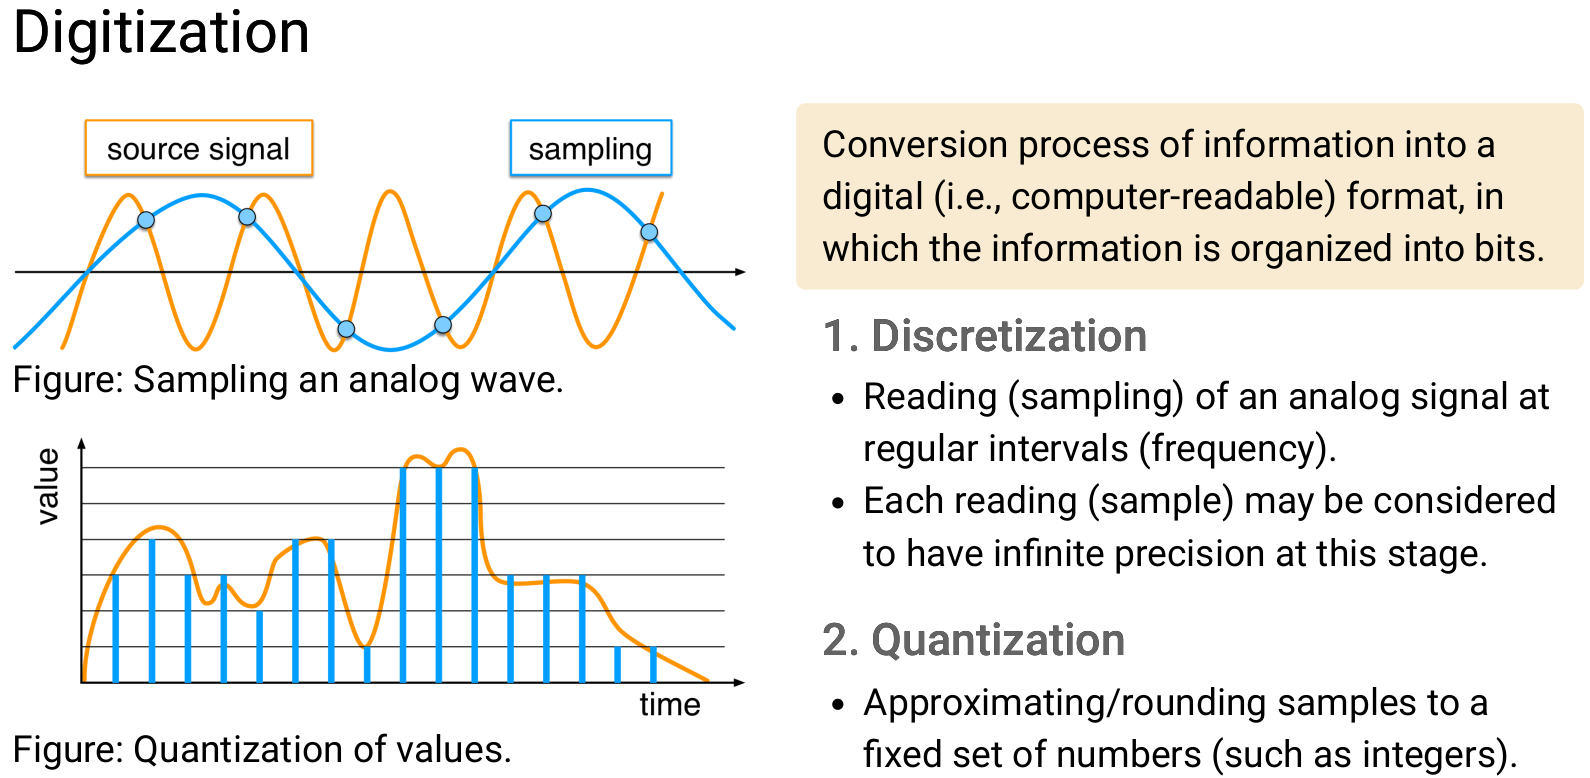
\includegraphics[width=\linewidth]{figures/digitalisierung.png}\\
	\textbf{Rastergrafik} Grafik wird als Pixel beschrieben, die jeweils eine Farbe haben $\rightarrow$ Skalierung schwierig. Beispiel: JPG, PNG, GIF, TIFF, PBM\\
	\textbf{Vektorgrafik} Inhalt der Grafik wird durch geometrische Formen beschrieben. Kann gerastert und beliebig skaliert werden. Beispiel: SVG, PS (Postscript), CGM, IGES, DWF/DXF\\


	\subsection{Menschliche Wahrnehmung von Licht}
	zwischen 380nm (violet/blau) und 780nm (rot)\\
	\textbf{Zapfen/Cones} Farbliche Wahrnehmung (ca. 6 Millionen) je für einen Farbkanal zuständig (64 \% rot, 32 \% grün, 4 \% blau)\\
	\textbf{Stäbchen/Rods} Helligkeitswahrnehmung (ca. 120 Millionen)\\
	\textbf{Farbsysteme} Repräsentation durch unterschiedliche Modelle, wie:
	\begin{itemize}
		\item biologisch orientiert: CIE XYZ
		\item Hardware-orientiert: RGB, CMY, CMYK (mit Schwarz, um Tinte zu sparen)
		\item Anwender-orientiert: HSV, HSB
	\end{itemize}
	\textbf{Steven's Power Law} physikalische Intensität (Helligkeit) ist nicht proportional zur wahrnehmbaren Helligkeit.\\
	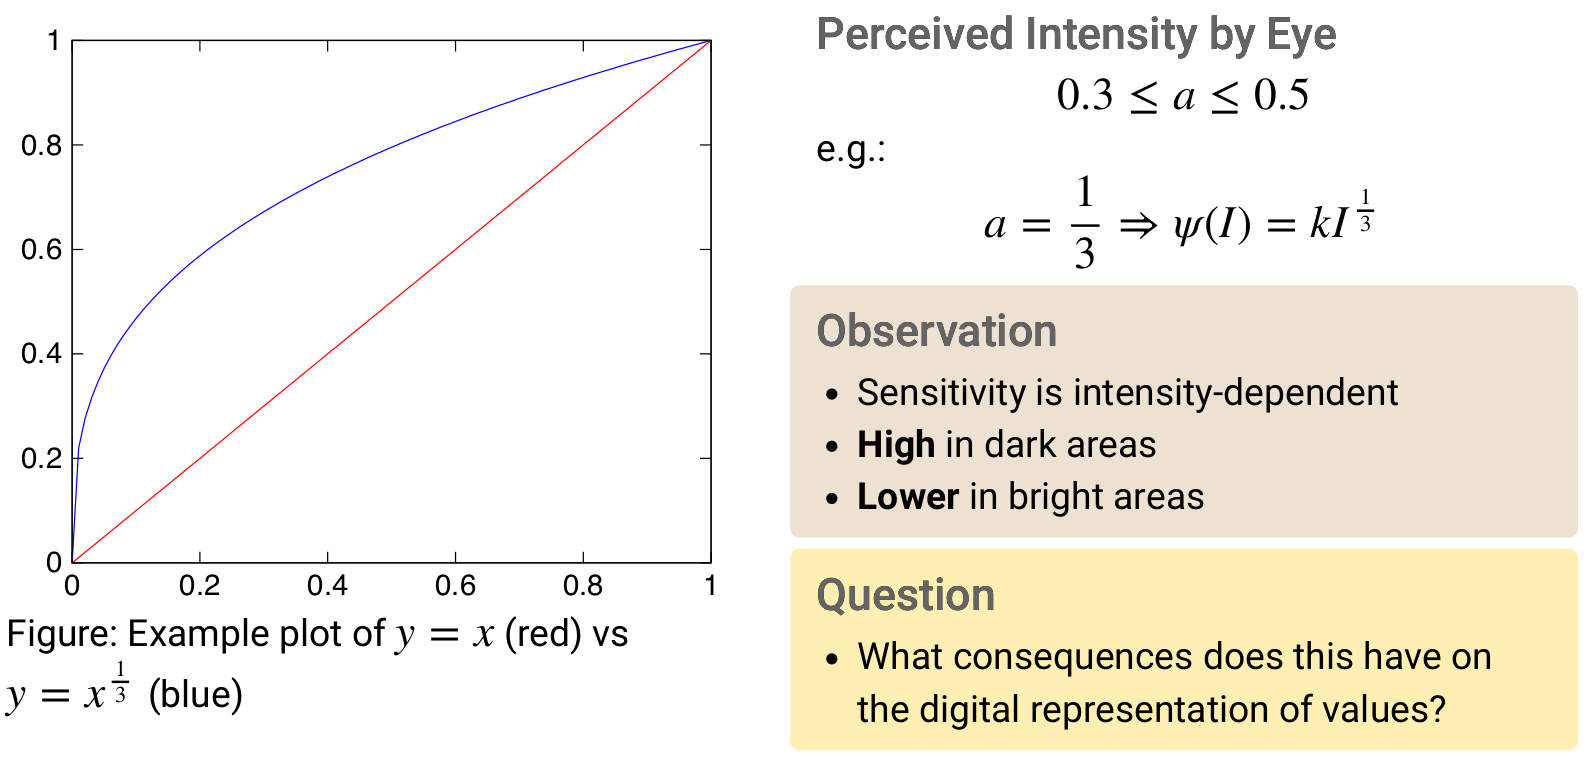
\includegraphics[width=\linewidth]{figures/stevens-law.png}\\
	\textbf{Gamma Korrektur} korrigiert physikalische Intensität, um kontinuierlichen wahrnehmbaren Intensitätszuwachs zu bekommen.\\
	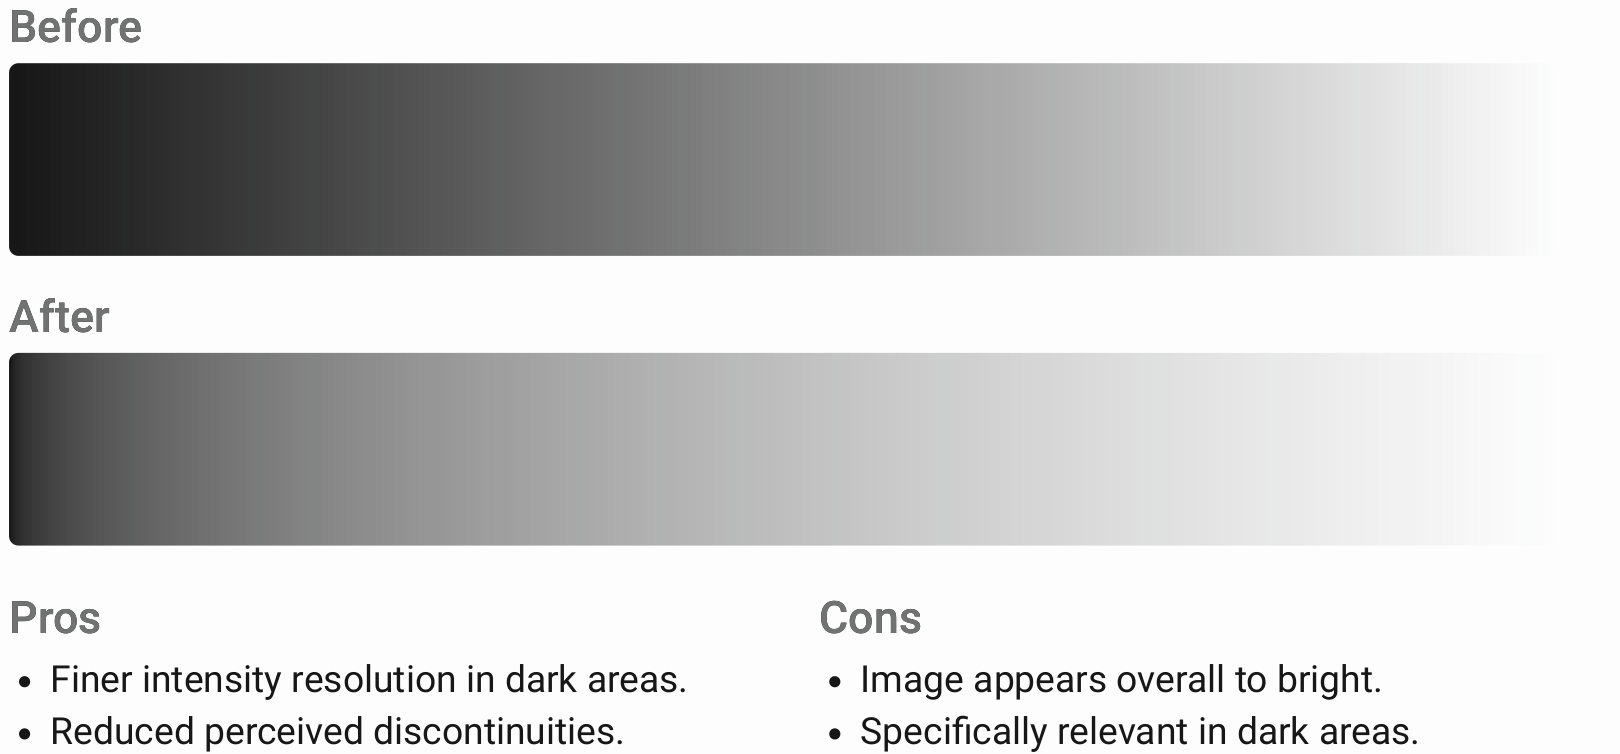
\includegraphics[width=\linewidth]{figures/gamma-correction.png}
	$$n = \lfloor I^{\frac{1}{\gamma}} 2^N \rfloor$$
	mit $I \in [0,1]$, $n \in [0,2^N]$: Abbildung der physikalischen Intensität auf wahrnehmungskorrigierte mit $N$ Bit Genauigkeit.

	\subsection{Rasterisierung von Vektorgrafiken}
	\textbf{Digital Differential Analyzer (DDA)} Rastern von Linien zwischen zwei beliebigen Punkten $p_1$ und $p_2$. Linie kann als Funktion $y = mx + b$ repräsentiert werden.\\
	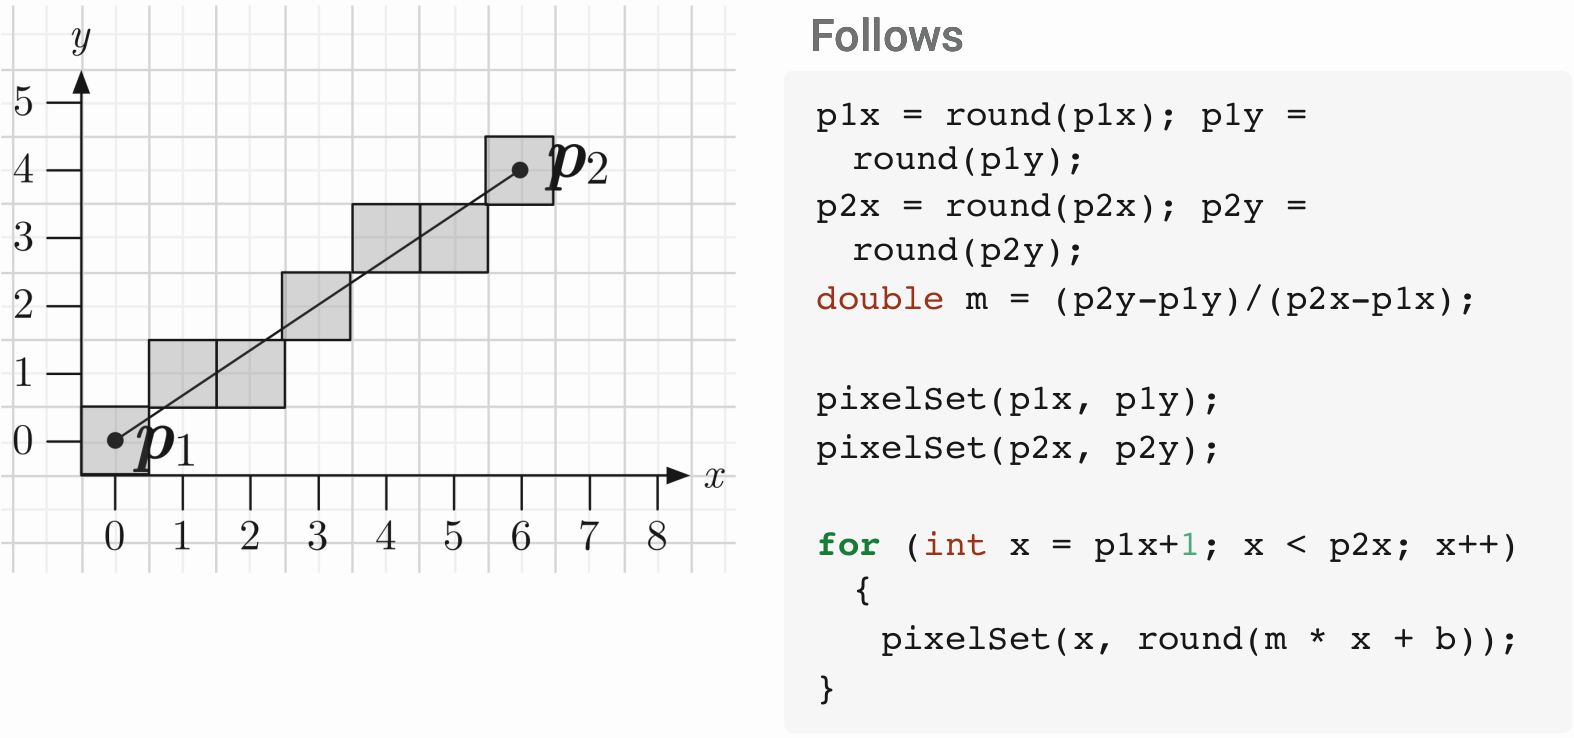
\includegraphics[width=\linewidth]{figures/dda.png}\\
	\textbf{Bresenham's Algorithmus} Verfeinerung von DDA\\
	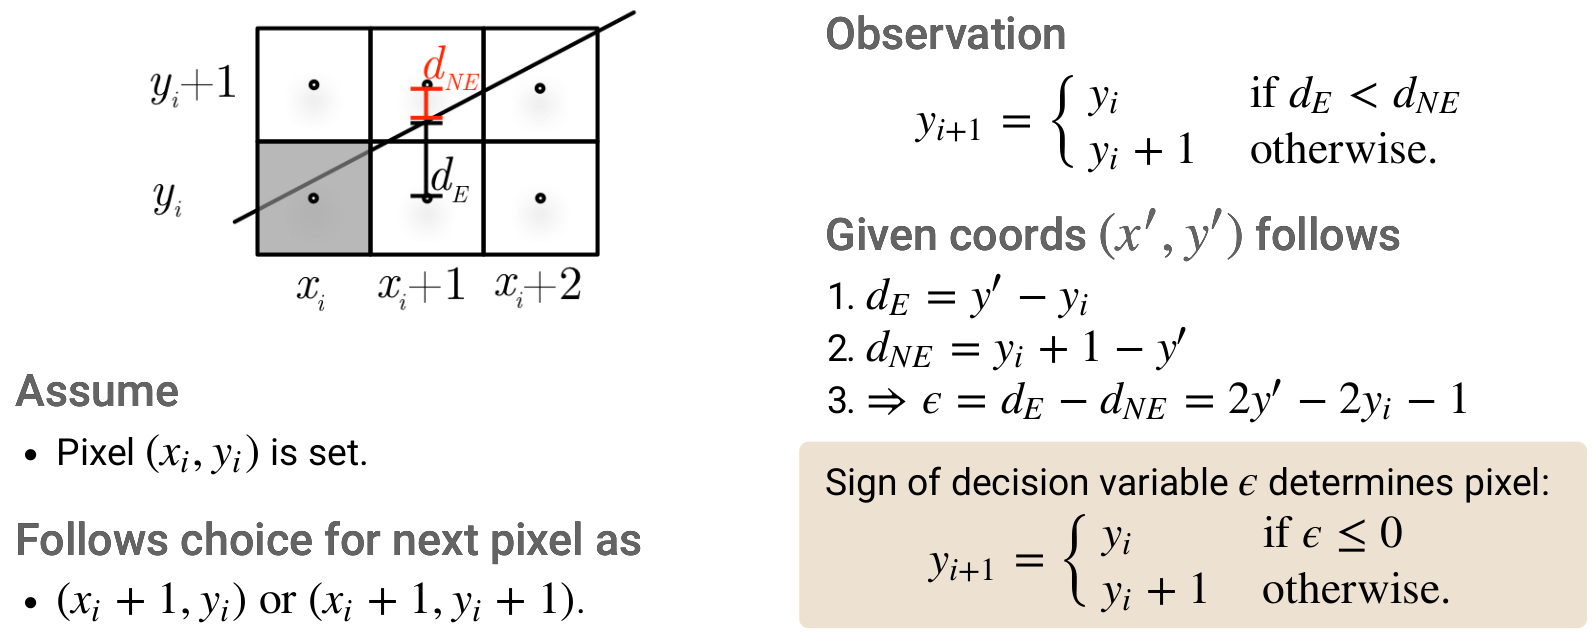
\includegraphics[width=\linewidth]{figures/bresenham.png}\\
	\textbf{Aliasing} Da Pixel entweder an oder aus sind (haben Farbe oder nicht), bildet sich eine Treppe beim Rastern von Linien. Kann beim Samplen auftreten\\
	$\rightarrow$ \textbf{Nyquist-Shannon Sampling Theorem} Sample Frequenz $>=$ Doppelte Signal Frequenz\\
	$\Rightarrow$ \textbf{Antialiasing} hat keine harten Übergänge sondern bildet "Farbverlauf" am Kantenrand (Pixel sind an, aus oder abgeschwächt farbig) durch Supersampling (mehr Punkte als Raster berechnen) und Durchschnittsbildung\\
	\textbf{Supersampling} feinere Auflösung als Zielbild wählen und regelmäßig samplen (beste Ergebnisse), zufällige Punkte wählen im gesamten Bild, zufällige Punkte in definierten Räumen

	\subsection{Vektoren}
	\textbf{Skalarprodukt/Dot-Produkt} $u \cdot v = (u_0, u_1, u_2)^T \cdot (v_0, v_1, v_2)^T = u_0 v_0 + u_1 v_1 + u_2 v_2$\\
	\textbf{Vektorlänge} $||v|| = \sqrt{v \cdot v}$\\
	\textbf{Kreuxprodukt} $w = u \times v = 
		\begin{bmatrix}
			u_1 v_2 - u_2 v_1\\
			u_2 v_0 - u_0 v_2\\
			u_0 v_1 - u_1 v_0
		\end{bmatrix}$\\
	$w$ ist orthogonal zu $u$ und $v$. Sie bilden ein rechthand-(Koordinaten)-System

	\subsection{Homogene Koordinaten}
	Repräsentieren von Vektoren als homogen, um Transformationen durchführen zu können. (wie in Robotik 1). Vierte Komponente ist 0 für Vektoren, 1 für Punkte.\\
	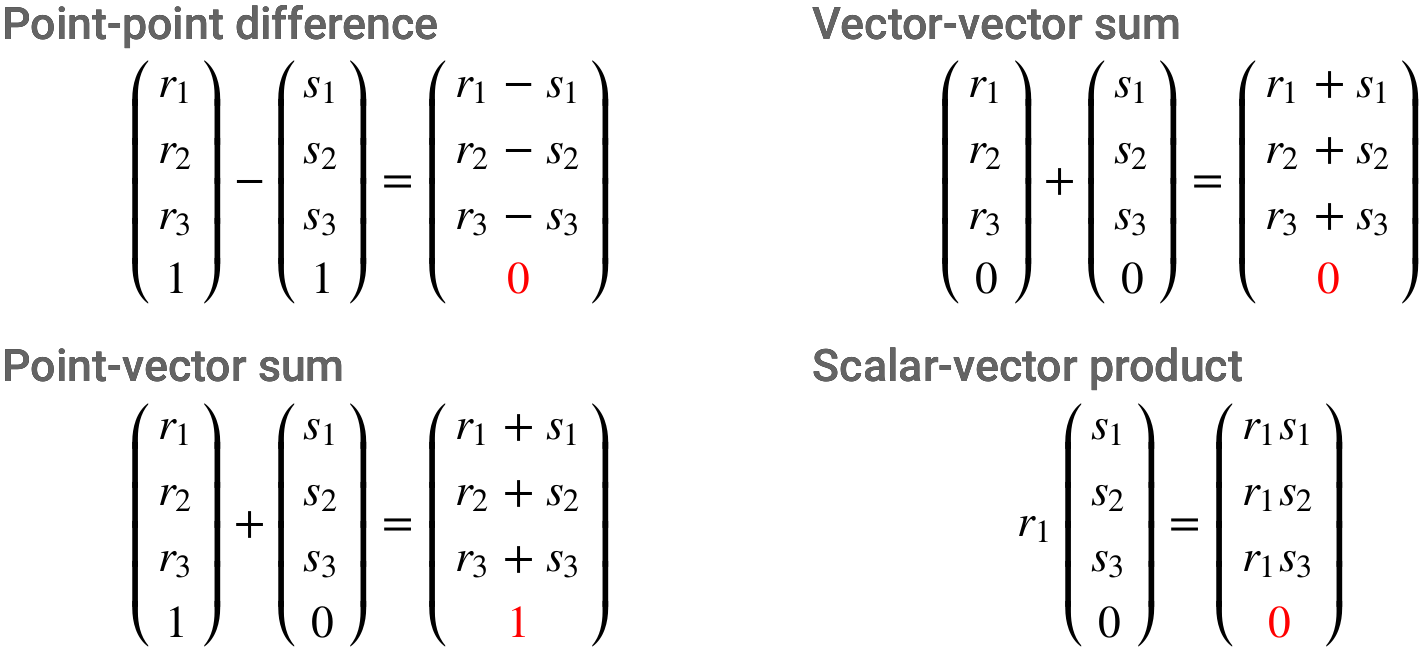
\includegraphics[width=\linewidth]{figures/homogene-koordinaten.png}
	\paragraph{Fundamental rotation matrices} $R_{n}(\phi)$ describes the rotation around the n axes with the angle $\phi$.\\
	\begin{equation}
	R_{1}(\phi) = 
	\begin{bmatrix}
	1 & 0 & 0\\
	0 & \cos \phi & -\sin \phi\\
	0 & \sin \phi & \cos \phi
	\end{bmatrix}
	\end{equation}
	\begin{equation}
	R_{2}(\phi) = 
	\begin{bmatrix}
	\cos \phi & 0 & \sin \phi\\
	0 & 1 & 0\\
	-\sin \phi & 0 & \cos \phi
	\end{bmatrix}
	\end{equation}
	\begin{equation}
	R_{3}(\phi) = 
	\begin{bmatrix}
	\cos \phi & -\sin \phi & 0\\
	\sin \phi & \cos \phi & 0\\
	0 & 0 & 1
	\end{bmatrix}
	\end{equation}
	
	\paragraph{Euler Angles transformation} Rotate around $m^3$ with $\theta_{1}$, $m^1$ with $\theta_{2}$ and $m^2$ with $\theta_{3}$ 
	\begin{equation}
	R_{3}(\theta_{1}) R_{1}(\theta_{2}) R_{2}(\theta_{3})
	\end{equation}
	
	\paragraph{Homogenous transformation} Describe coordinates as homogenous coordinates to describe rotations and translations\\
	vector $q$ as homogenous coordinates is $[q_{1} q_{2} q_{3} 1]^T$\\
	Homogenous transformation matrix
	\begin{equation}
	T = 
	\begin{bmatrix}
	R & p\\
	\eta^T & 1
	\end{bmatrix}
	\end{equation}
	with\\
	$R \in \R^{3 \times 3}$ is a rotation matrix\\
	$p \in \R^{3 \times 1}$ is a translation vector\\
	$\eta^T \in \R^{1 \times 3}$ is a perspective vector, here zero vector
	\begin{equation}
	Rot(\phi, k) = 
	\begin{bmatrix}
	& & & 0\\
	& R_{k}(\phi) & & 0\\
	& & & 0\\
	0 & 0 & 0 & 1
	\end{bmatrix}, 
	Tran(p) = 
	\begin{bmatrix}
	1 & 0 & 0 & p_{1}\\
	0 & 1 & 0 & p_{2}\\
	0 & 0 & 1 & p_{3}\\
	0 & 0 & 0 & 1
	\end{bmatrix}
	\end{equation}
	Calculate arbitrary transformations by using the following rules:
	\begin{enumerate}
		\item Start with $T = I$, $F$ (fixed frame) and $M$ (mobile frame) are equivalent
		\item Represent rotations and translations as separate fundamental homogenous transformation matrices
		\item If $M$ is rotated about or translated along a unit vector of $F$, \textbf{premultiply} homogenous transformation matrix to $T$
		\item If $M$ is rotated about or translated along a unit vector of $M$, \textbf{postmultiply} homogenous transformation matrix to $T$
	\end{enumerate}
	This results in the matrix $T_F^M$ mapping coordinates from the mobile coordinate frame $M$ to the fixed one $F$:
	$$[p]^F = T_F^M [p]^M$$
	
	\paragraph{Reflection} Use identity matrix with $-1$ for the reflection axis. Reflection at a point is reflection at the intersection of three orthogonal planes ($-1$ for every axis).

	\paragraph{Transformation for abitraty points} Translate everything so that the transformation point is located at the origin. Do the Transformation. Translate everything back.
	
	\paragraph{Inverse homogenous transformation} If the transformation matrix $T$ maps coordinates from coordinate frame $A$ to $B$, the inverse $T^{-1}$ maps coodinates from $B$ to $A$.
	\begin{equation}
	T^{-1} = 
	\begin{bmatrix}
	& R^T & & -R^T p\\
	0 & 0 & 0 & 1
	\end{bmatrix}
	\end{equation}
	with $\eta = 0$ and $\sigma = 1$
	
	\section{Raytracing}
	Rendern von 3D-Objekten als 2D-Repräsentation. Orientiert an Physik, dadurch sehr realistische Darstellungen möglich. Strahlen werden von Kamera in die Szene gesendet. Schneiden diese ein 3D-Objekt, wird der Strahl von dort zu einer Lichtquelle verfolgt und der aussendende Pixel entsprechend gefärbt.\\
	\begin{verbatim}
		raytrace(scene, camera, image):
		   # For all pixels in image
		   for (x, y) in image:
		      # 1. Generate ray through pixel
		      ray = camera.generateRay(x, y)
		      # 2. Find closest intersection with scene
		      hit = scene.intersect(ray)
		      # 3. Calculate light intensity
		      color = shade(hit, scene)
		      # 4. Set pixel color
		      image.set(x, y, color)		
	\end{verbatim}
	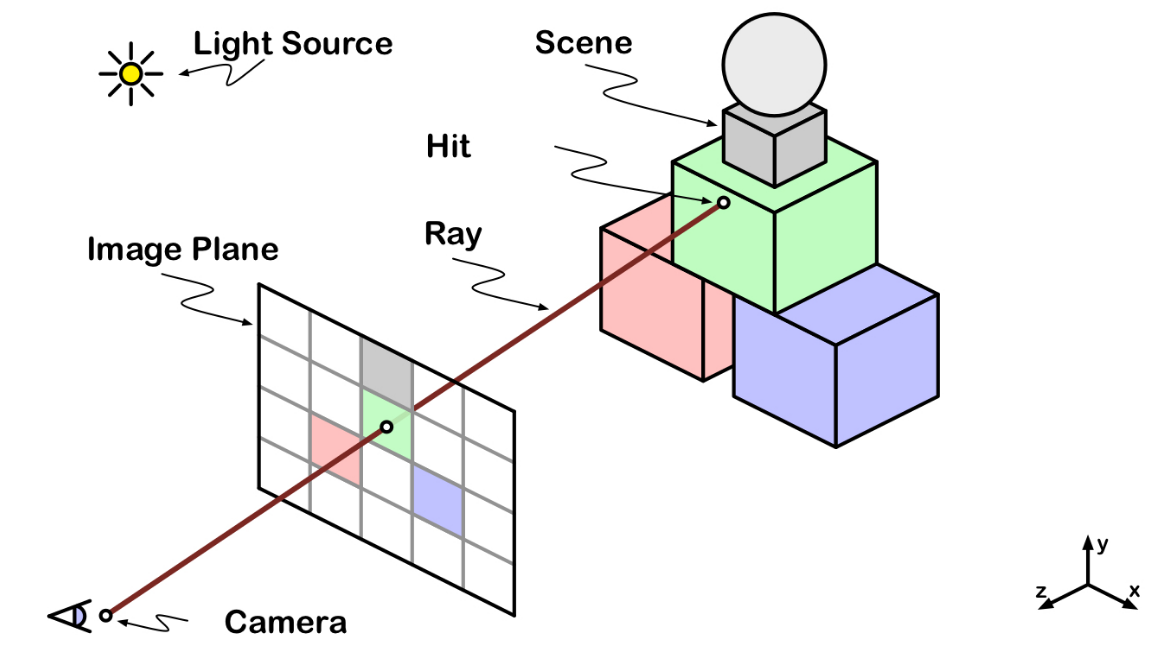
\includegraphics[width=\linewidth]{figures/raytracing.png}\\
	\textbf{Photon} Lichtstrahl mit bestimmter Energie bzw. Farbe
	$$E = h \cdot f$$
	mit $E$: Energie, $h$: Planksche Konstante, $f$: Frequenz
	$$1 Lumen = 4 \cdot 10^{15} Photonen/sec$$
	\textbf{Absorption} Photon verschwindet, wird von Gegenstand geschluckt\\
	\textbf{Reflektion} Photon prallt an Oberfläche ab\\
	\textbf{Refraktion} Photon geht durch eine Oberfläche hindurch (z.B. Glas)\\
	\textbf{Ray/Strahl} Dargestellt als Startpunkt mit Richtungsvektor: $x(t) = x_0 + t \vec{d}$
	\textbf{Licht-Material Interaktion} Mögliche Modelle zur realistischen Farbermittlung:
	\begin{itemize}
		\item Quantum Theorie (Emission, Absorption)
		\item Spezielle Relativität (aberration, blueshift, redshift, time dilatation)
		\item Wellenoptik (diffraction, dispersion, Interferenz)
		\item Geometische Optik (Reflektion, Refraktion)
	\end{itemize}

	\subsection{Shading}
	Verwende Objektfarbe bei Rayintersection. Naiver Ansatz, da physikalische Gesetze wie Reflektion oder Schatten und Objektstruktur ignoriert werden. Gleichmäßig gefärbte Objekte.

	\subsection{Phong Relektionsmodell}
	Modell zur Farbberechnung. Basiert auf geometischer Optik. Setzt sich zusammen aus der Farbe (Ambient) + Oberflächenbeschaffenheit und Schatten (Diffuse) + Reflektion (Specular). Verwendet folgende Vereinfachungen:
	\begin{itemize}
		\item Oberfläche: Isotropic, betrachtet nicht die Wellenlänge und Polarisierung
		\item Raum: nimmt Vacuum an, keine atmospherischen Effekte
		\item Licht: Lichtquellen als einzelne Punkte
	\end{itemize}
	\textbf{Ambient}\\
	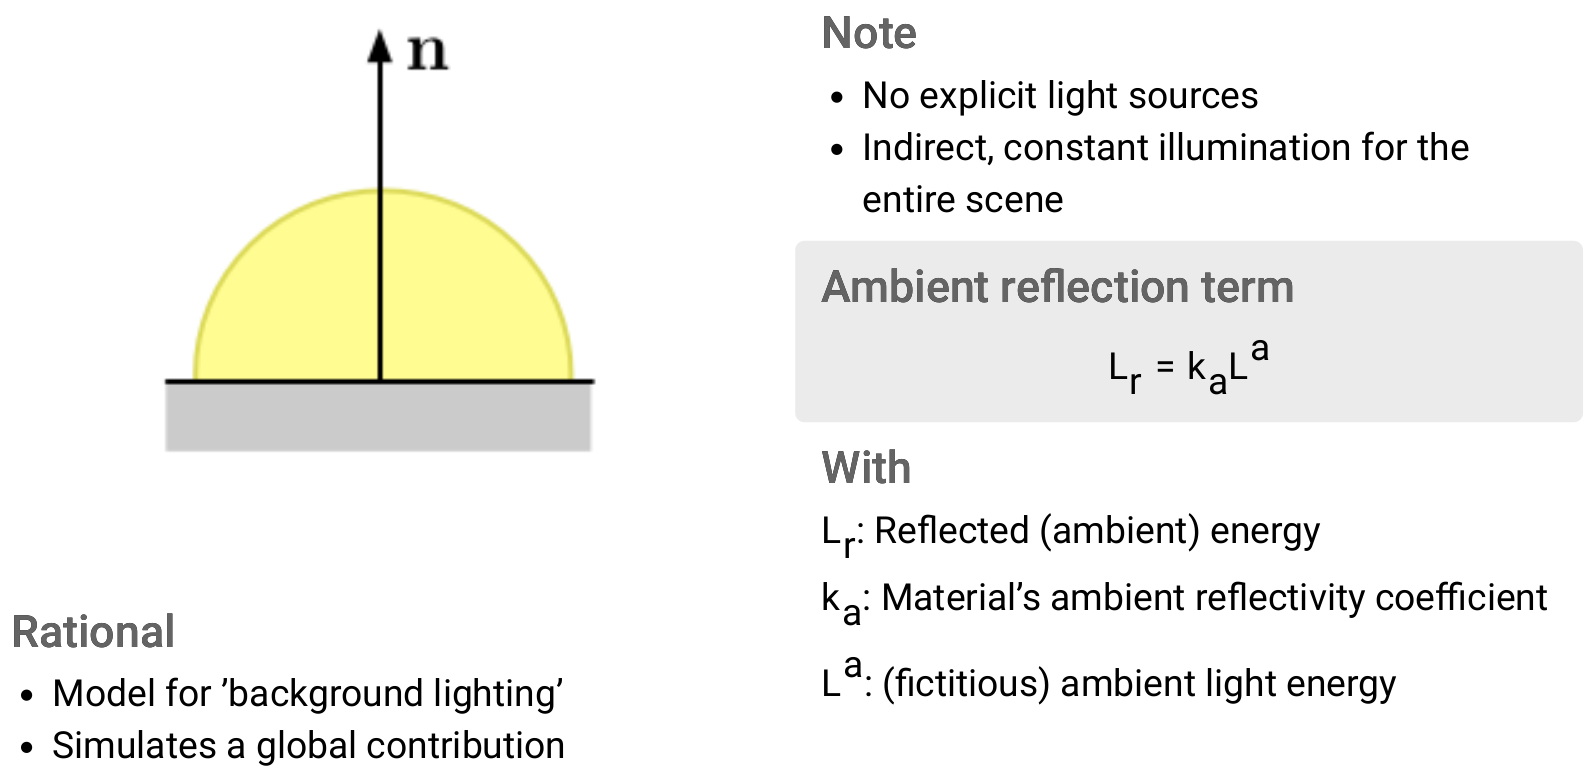
\includegraphics[width=\linewidth]{figures/phong-ambient.png}\\
	\textbf{Diffuse} Betrachtet reflektiertes Licht von Oberflächen (unterschiedlich je nach Oberfläche matt/glänzend)\\
	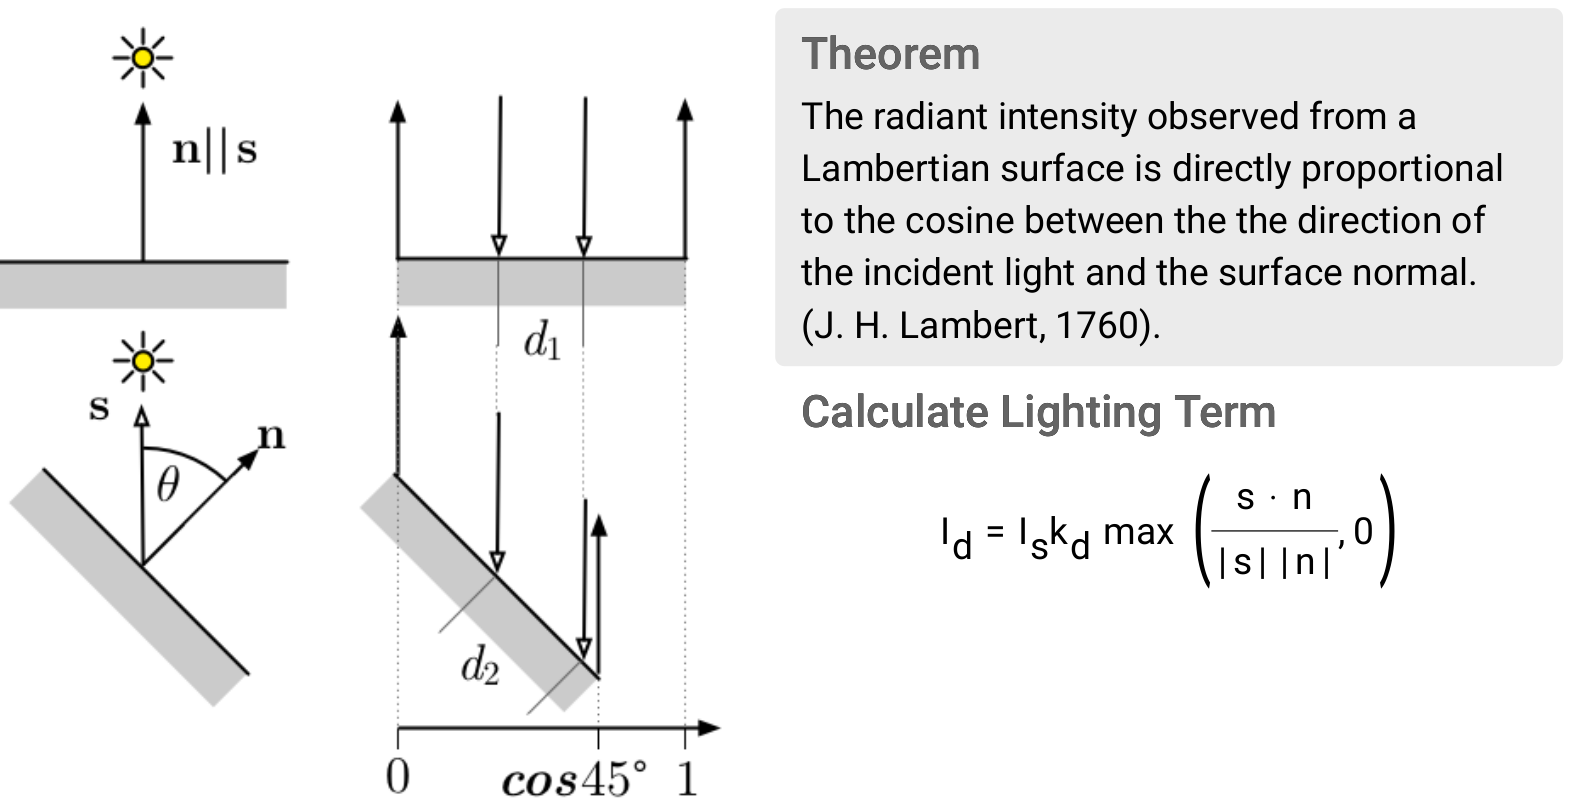
\includegraphics[width=\linewidth]{figures/phong-diffuse.png}
	$$L_d(p) = k_d \sum_j L_j \max(0, n \cdot s_j)$$
	mit $L_d$: Reflektiertes Licht (Diffuse-Anteil)\\
	$k_d$: Material-Koeffizient für Diffuse Reflektion\\
	$L_j$: Licht (Farbe) der Lichtquelle $j$\\
	$n$: Normale vom Punkt $p$ zur Oberfläche\\
	$s_j$: Vektor von $p$ zur Lichtquelle $j$\\
	\textbf{Specular} Betrachtet starke Reflektionen für glänzende Oberflächen (weiße/helle Punkte)\\
	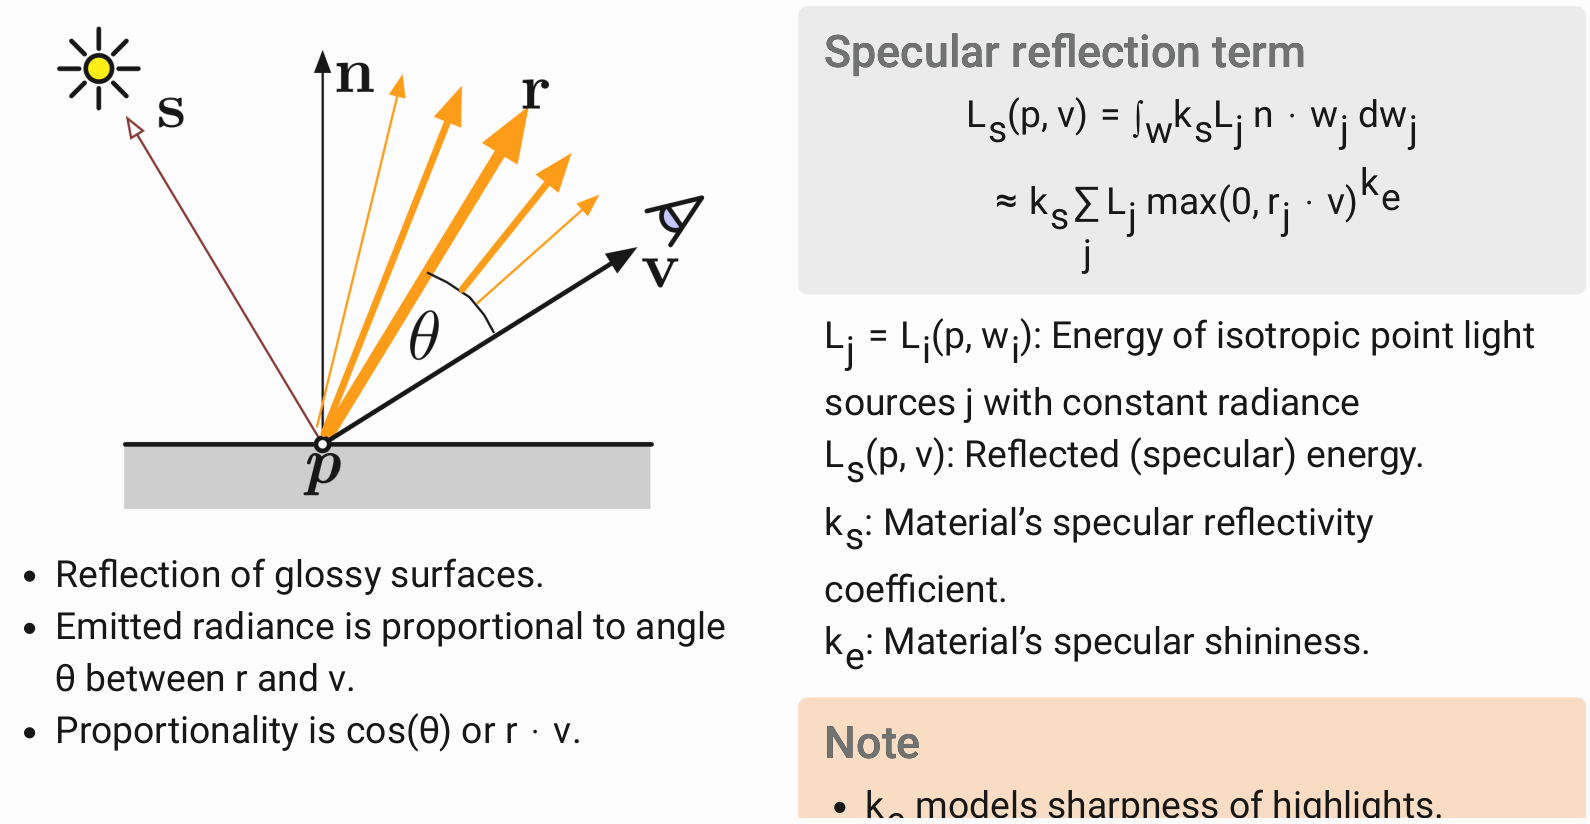
\includegraphics[width=\linewidth]{figures/phong-specular.png}\\
	\textbf{Reflektionsberechnung} Berechnung des Reflektionsvektors\\
	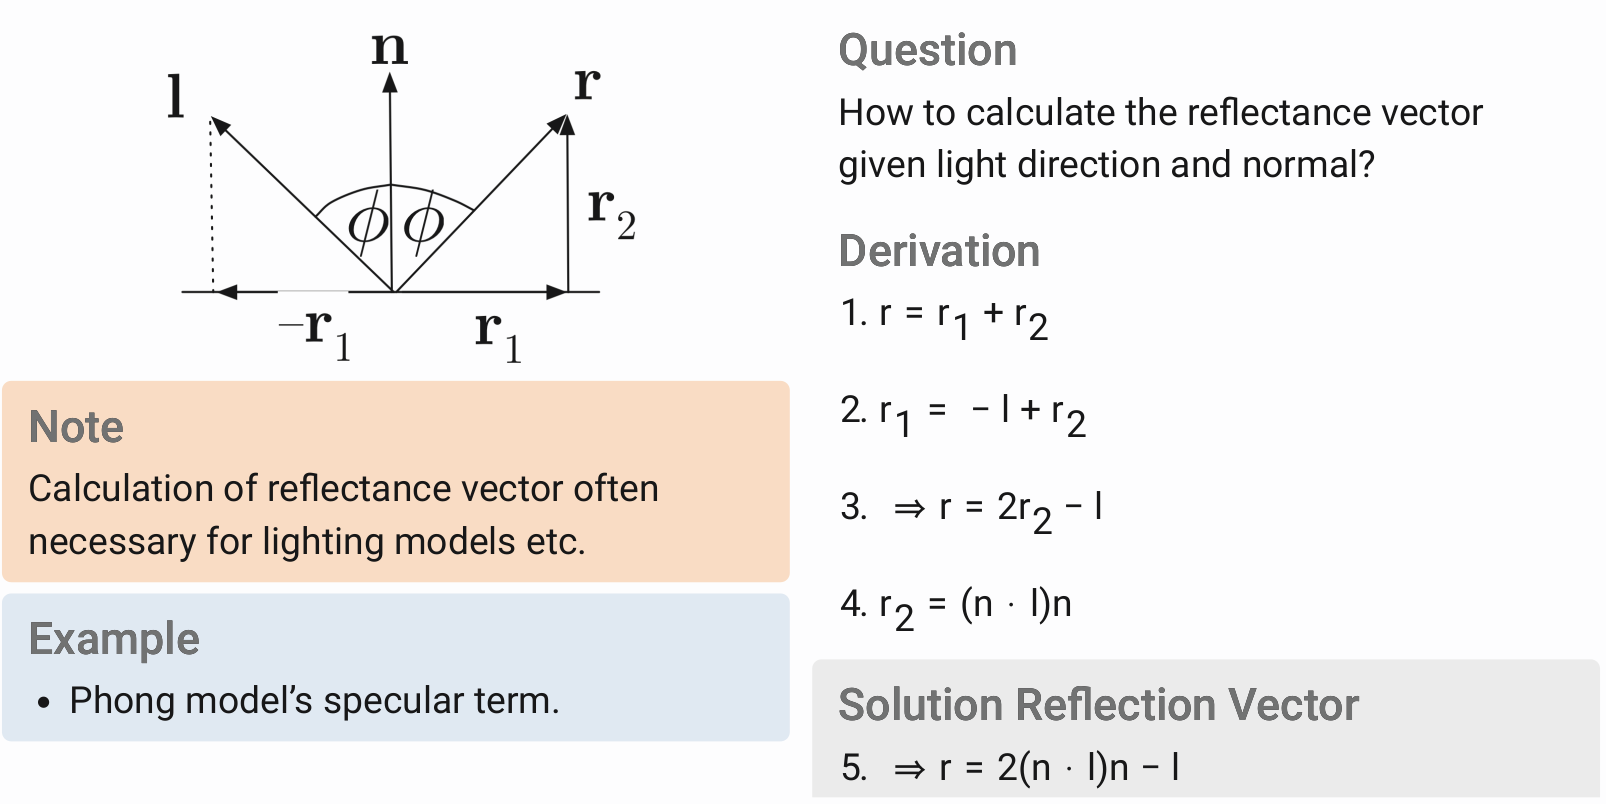
\includegraphics[width=\linewidth]{figures/reflektionsvektor.png}

	\section{Scene Graph}
	Ein Szenengraph repräsentiert alle Objekte einer Szene als Graph. Dabei werden Positionen immer relativ zum Elternelement angegeben. Wird eine globale Position relativ zum Weltkoordinatensystem benötigt, müssen alle Transformationen entlang des Graphs vom Ursprung zum Objekt angewendet werden.\\
	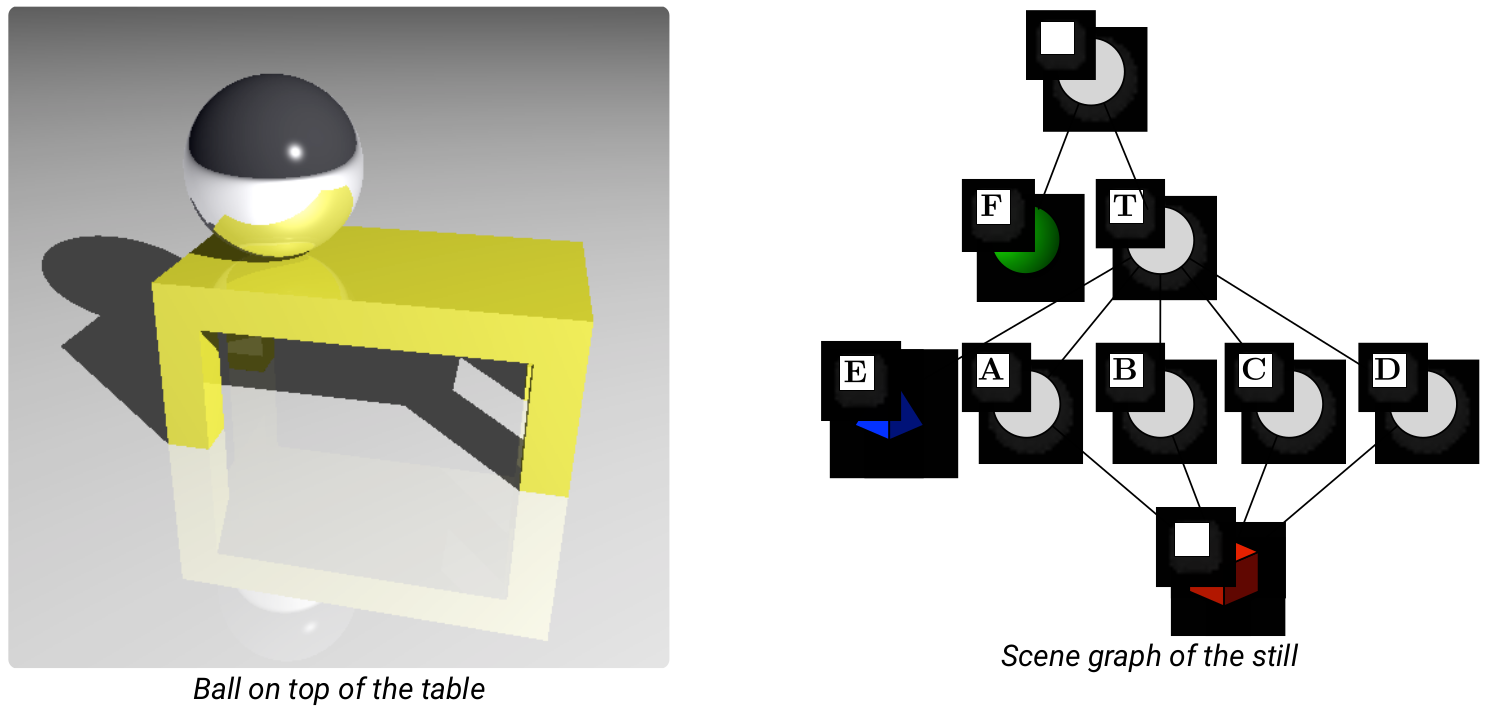
\includegraphics[width=\linewidth]{figures/scene-graph.png}

	\subsection{Koordinatensysteme}
	Man unterscheidet mehrere Koordinatensysteme\\
	\textbf{Weltkoordinatensystem $\mathbf{W}$} Globales Referenzsystem für alle Objekte\\
	\textbf{Objektsystem $\mathbf{O}$} Relatives System für jedes Objekt. Urspung im Objektursprung. Verwendet z.B. um Punkte eines Objekts relativ zum Ursprung anzugeben.\\
	\textbf{Kamerasystem $\mathbf{C}$} System relativ zur Kameraposition

	\subsection{Rendering}
	Zum Rendern des Scene-Graphs wird das Visitor-Pattern verwendet.\\
	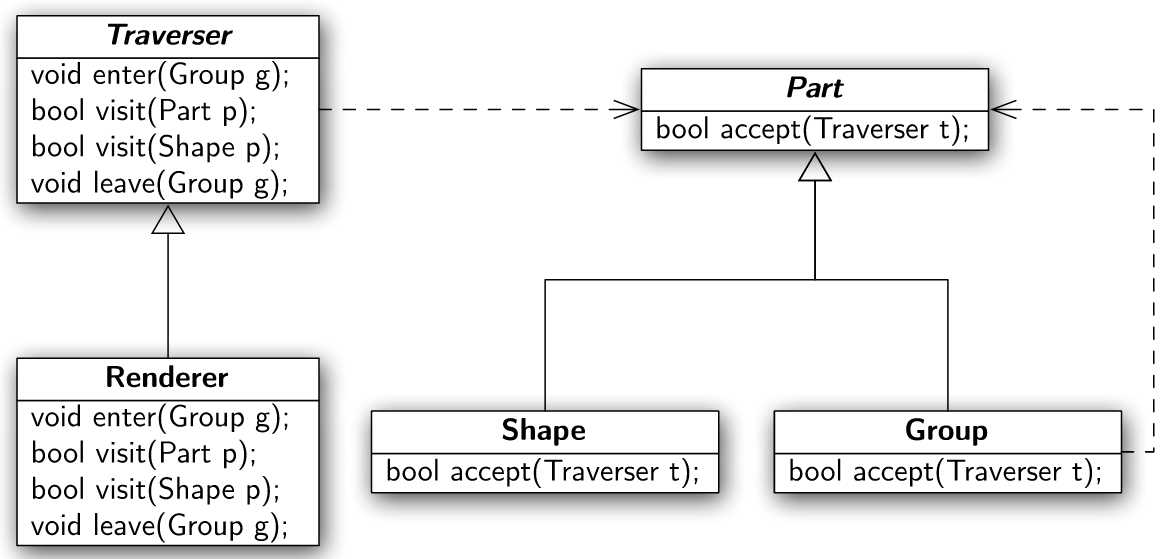
\includegraphics[width=\linewidth]{figures/visitor-pattern.png}

	\section{Rasterisierung}
	Abbildung von 3D-Objekten auf 2D-Projektionsfläche $\rightarrow$ Forward Rendering\\
	\textbf{Unterschied zu Raytracing} Szene wird auf Betrachter projektiert. Bei Raytracing wird vom Betrachter aus die Szene mit Rays abgetastet, dadurch flexibler. Rasterisierung ist an geometische Formen und deren 2D-Abbildung gebunden, dadurch aber schneller.
	
	\subsection{Pipeline}
	Ablauf der Rasterisierung lässt sich gut durch Pipeline darstellen, deren Schritte durchlaufen werden:\\
	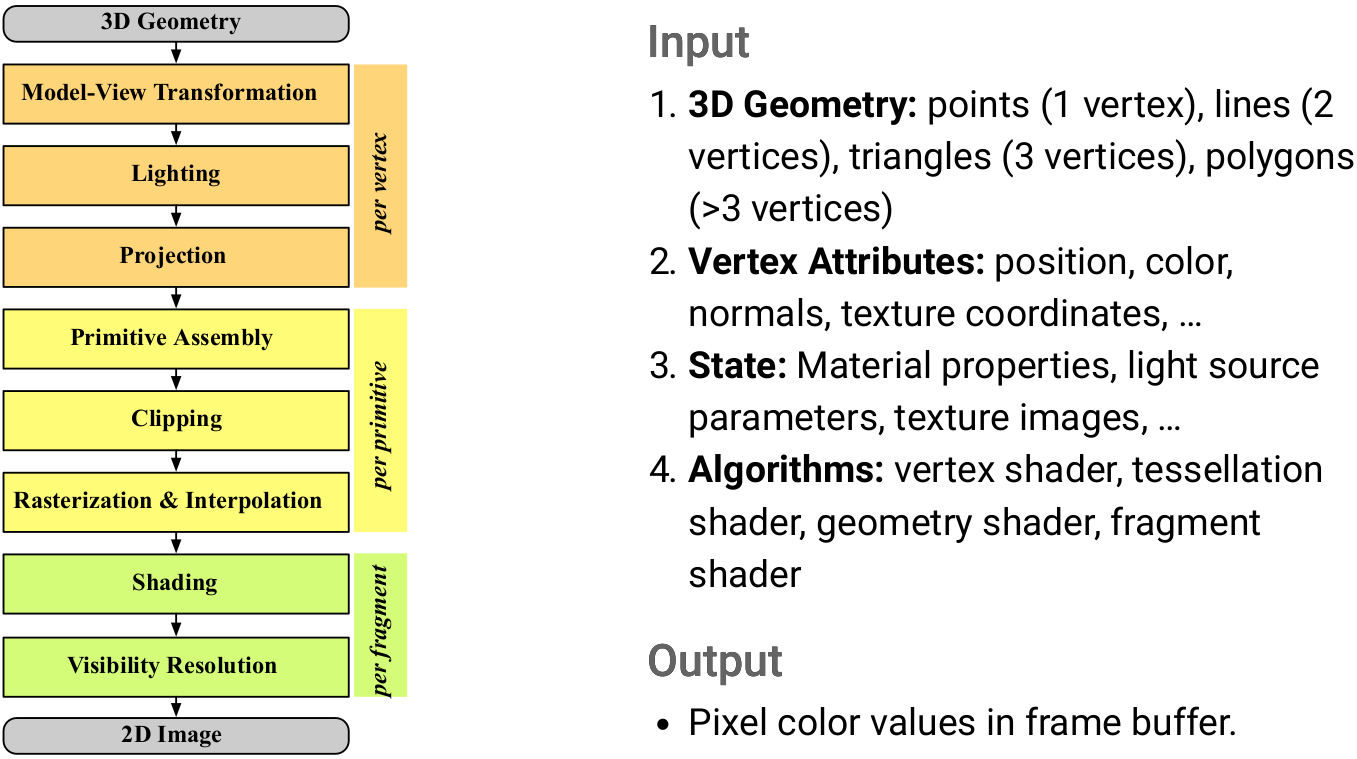
\includegraphics[width=\linewidth]{figures/rasterization-pipeline.png}\\
	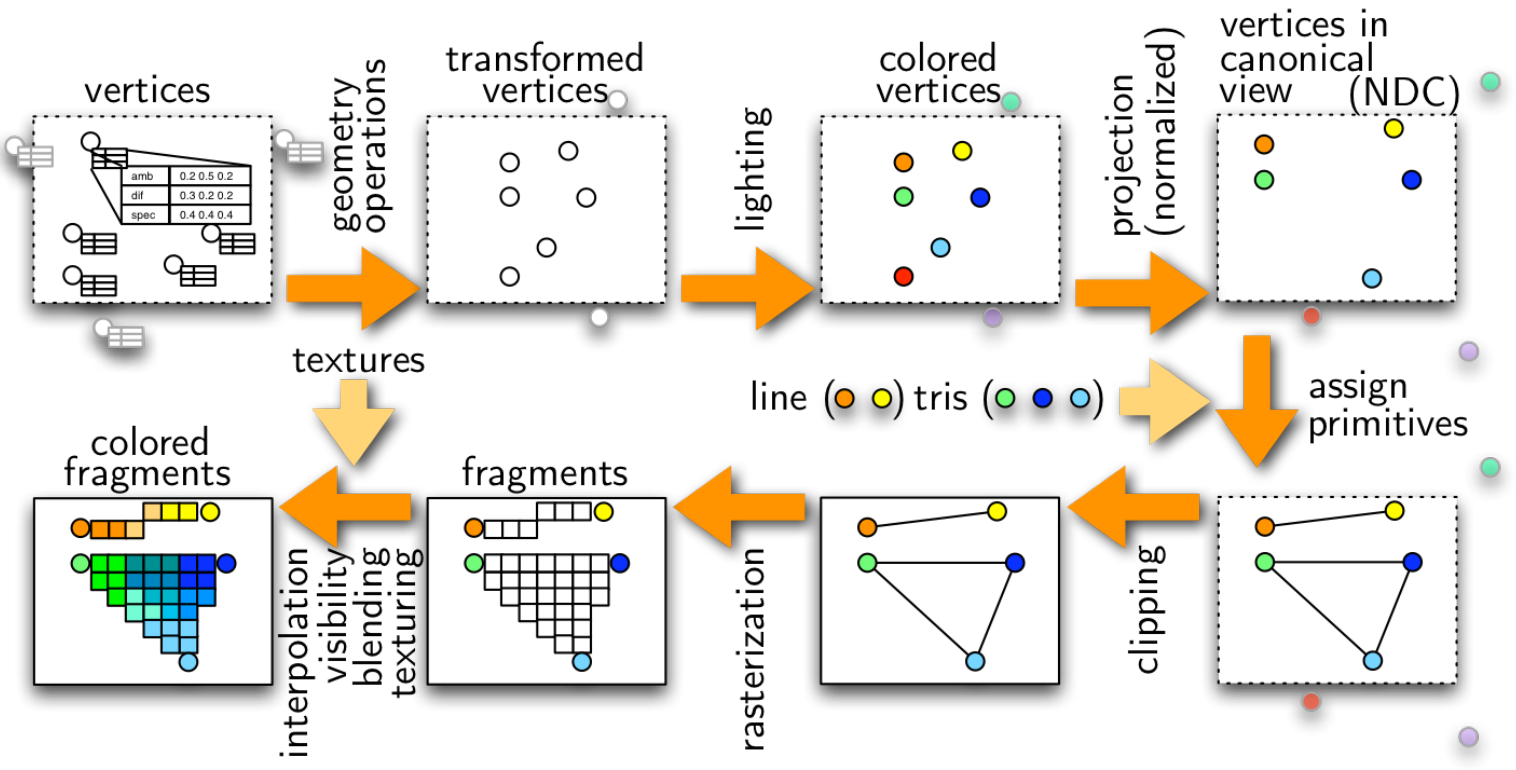
\includegraphics[width=\linewidth]{figures/rasterization-pipeline2.png}\\
	\textbf{Model-View Transformation} Transformiert die 3D-Objekte von den Objektsystemen in das Kamerasystem (analog Scene Graph)\\
	\textbf{Lightning} Bestimmt die Farben der 3D-Objekte (z.B. mit Phong)\\
	\textbf{Projection} Bestimmt den Bereich, der durch die Projektionsfläche abgebildet werden kann. Dabei wird die Projektionsmatrix auf die Geometriedaten angewendet.\\
	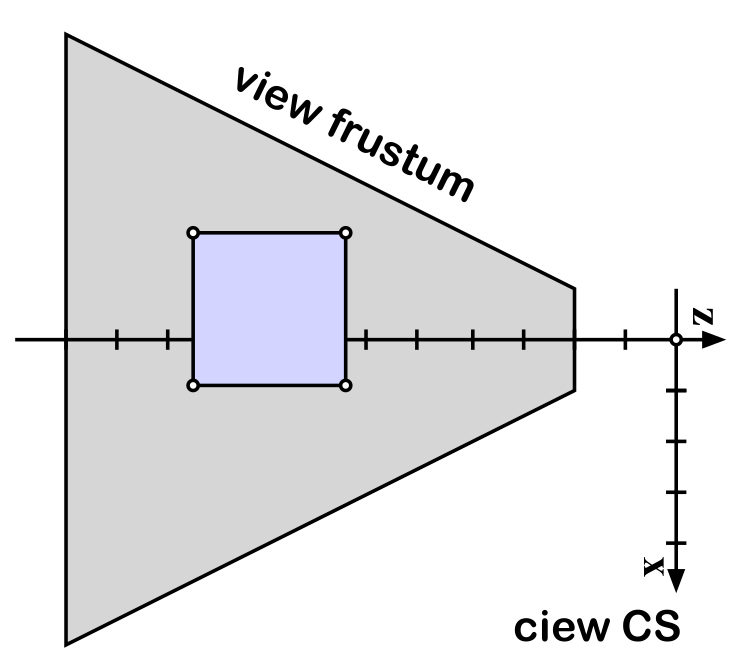
\includegraphics[width=0.5\linewidth]{figures/rasterization-projection1.png}
	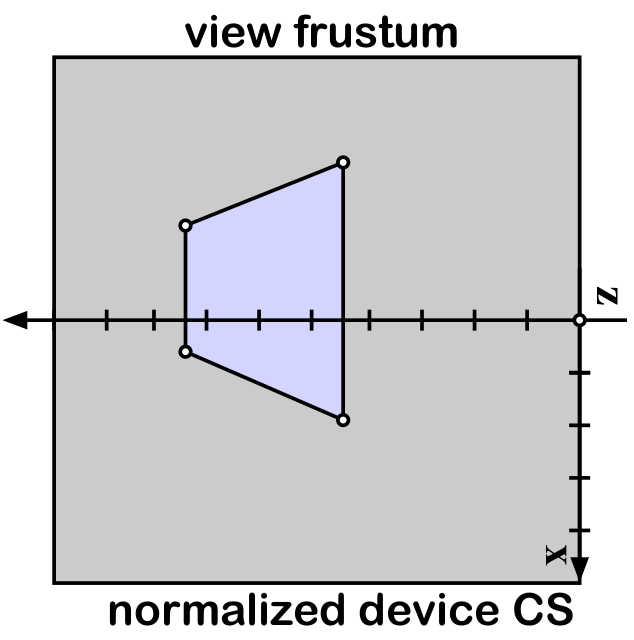
\includegraphics[width=0.5\linewidth]{figures/rasterization-projection2.png}\\
	\textbf{Primitive Assembly} Gruppiert Vertices zu Primitives wie Punkt, Linie oder Dreieck. Benötigt dafür die Information, welche Vertices zusammen gehören.\\
	\textbf{Clipping} Schneidet vorhandene Primitives zu anhand des vorher bestimmten sichtbaren Projektionsbereichs. Dabei können Primitives komplett verschwinden oder verändert werden, wenn Teile davon außerhalb der Projektionsfläche liegen.\\
	\textbf{Rasterization \& Interpolation} Generiere Attribute (wie Farbe) für Werte (Pixel), die innerhalb von Primitives liegen (z.B. das Innere vom Dreieck). Dies geschieht durch Interpolation der Eckpunkte der Primitives. Dabei entsteht für jedes Primitive ein Stream an Fragments (Position und Farbe), der diese Informationen speichert.\\
	\textit{Fragmente} gehören immer zu einem Pixel. Es kann allerdings mehrere Fragmente pro Pixel geben, wenn z.B. Multisampling durchgeführt wird. Allerdings gibt es mindestens ein Fragment pro Pixel.\\
	\textbf{Shading} Mappt die einzelnen Fragments auf die Farben der Pixel. Es entsteht ein Stream mit $0..n$ Farbwerten.\\
	\textbf{Visibility Resolution} Prüft die Tiefenwerte der Fragmente und füllt den z-Buffer. Dieser gibt an, wie weit ein Pixel/Fragment von der Projektionsfläche nach hinten entfernt liegt.

	\subsection{Zusammenfassung}
	Da die einzelnen Schritte der Pipeline klare Schnittstellen haben, können diese als Black-Boxes angesehen werden und individuell implementiert werden.\\
	\textbf{Vertex Shader} Die Verarbeitung von Vertices wird Vertex Shader genannt.\\
	\textbf{Fragment Shader} Die Verarbeitung von Framgents wird Fragment Shader genannt.

	\section{Viewing and Projection}
	Sehen ist die Abbildung einer 3D-Szene auf ein sichtbares 2D-Bild. Dabei spielt sowohl die Position der sichtbaren Objekte eine Rolle wie auch die Position des Betrachters (unterschiedliche Abbildungen je nach Blickwinkel).\\
	\textbf{Projektion} Mapping von einem höherdimensionalen Raum in einen niedriger dimensionierten Raum (z.B. 3D $\rightarrow$ 2D)\\
	\textbf{Projektoren} Pfade/Linien, die Objekte mit der Projektionsfläche verbinden und damit den Abbildungspfad aufzeigen. Sie gehen durch den COP oder parallel zum DOP.\\
	\textbf{Center of Projection (COP)} Punkt zu dem die Projektion durchgeführt wird (z.B. Auge, Kameraposition)\\
	\textbf{Direction of Projection (DOP)} vorgegebene Projektionsrichtung zu der alle Projektoren parallel sind $\rightarrow$ der angenommene COP liegt im unendlichen.\\
	\textbf{Projektionsfläche/Projection (View) Plane (PP/VP)} Fläche auf der die finale Projektion abgebildet wird. Das Zentrum der VP ist das VPC.

	\subsection{Lochkamera/Pinhole Camera}
	Einfache Abbildung von Lichtstrahlen, die durch Loch an der Vorderseite eintreten und auf Rückwand abgebildet werden.\\
	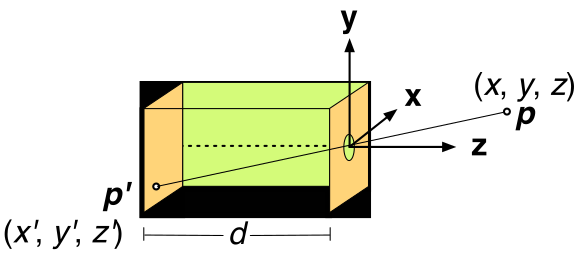
\includegraphics[width=0.5\linewidth]{figures/pinhole-camera1.png}
	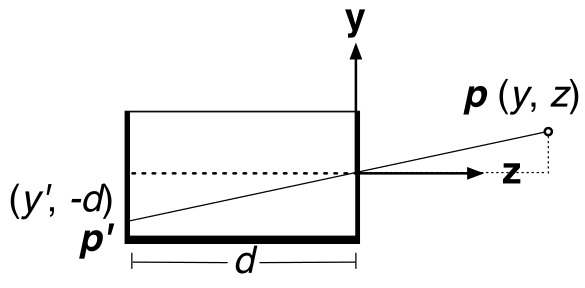
\includegraphics[width=0.5\linewidth]{figures/pinhole-camera2.png}
	$$z' = -d$$
	$$\frac{y'}{-d} = \frac{y}{z} \rightarrow y' = -\frac{y d}{z}$$
	$$\frac{x'}{-d} = \frac{x}{z} \rightarrow x' = -\frac{x d}{z}$$
	$$\gamma = \frac{\beta}{2}, \sin \gamma = \frac{h}{2a}, \cos \gamma = \frac{d}{a} \rightarrow \sin \gamma = \frac{h \cos \gamma}{2d} \Rightarrow \beta = 2 \tan^{-1} \frac{h}{2d}$$

	\subsection{Orthogonale Projektion}
	Projektion entlang einer DOP, die der z-Achse entspricht. Projektionsfläche bei $z=0$
	$$p' =
	\begin{bmatrix}
		p'_x\\
		p'_y\\
		p'_z\\
		1
	\end{bmatrix} = 
	\begin{bmatrix}
		p_x\\
		p_y\\
		0\\
		1
	\end{bmatrix} = 
	P_{ortho} p = 
	\begin{bmatrix}
		1 & 0 & 0 & 0 \\
		0 & 1 & 0 & 0 \\
		0 & 0 & 0 & 0 \\
		0 & 0 & 0 & 1
	\end{bmatrix}
	\begin{bmatrix}
		p_x\\
		p_y\\
		p_z\\
		1
	\end{bmatrix}
	$$

	\section{Animation}
	Viele, minimal abweichende Bilder nacheinander erzeugen die Illusion von Animation bzw. bewegten Bildern/Videos. Frames werden über Zeit gestaffelt, Animation muss zeitabhängige Funktion sein $\Delta t = t_x - t_{x-1}$, da dann auch unhabhängig von variabler Framerate.\\
	\textbf{Einfügen in Scene Graph} Animationsfunktion verändert Position einzelner Knoten abhängig von der Zeit\\
	\textbf{Lineare Interpolation} Berechnung von Zwischenschritten ohne Anwendung der Animationsfunktion. Möglich für Translation, da Elemente unabhängig voneinander sind. Nicht für Rotation, da Elemente der Rotationsmatrix voneinander abhängen (abhängig vom Rotationswinkel).

	\section{Quaternions}
	Repräsentation von Vektoren mit 4 Elementen in $\C$. Vereinfacht das Rechnen im Vergleich zu Rotationsmatrizen.\\
	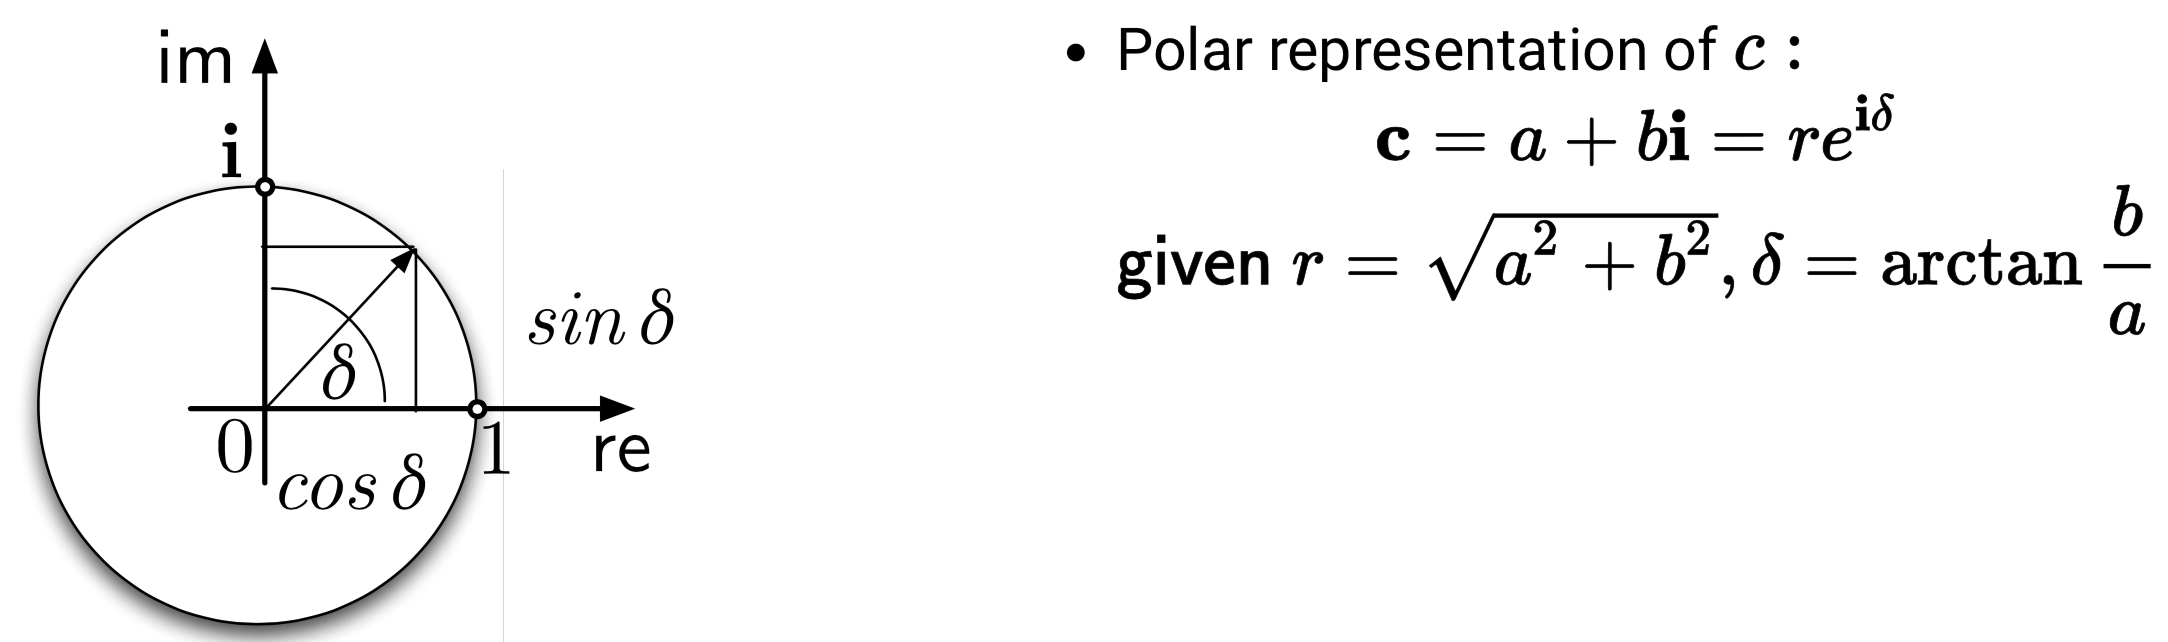
\includegraphics[width=\linewidth]{figures/2d-complex-coordinates.png}\\
	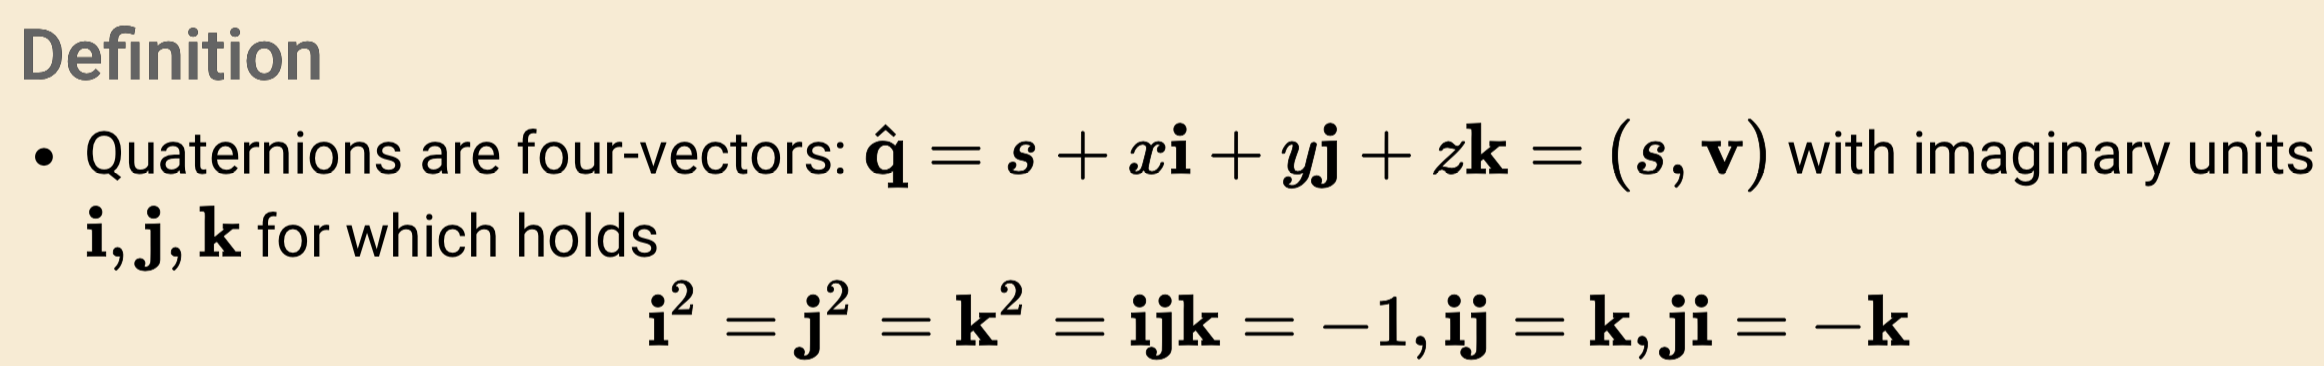
\includegraphics[width=\linewidth]{figures/quaternions.png}
\end{document}
